\documentclass{cards}

\begin{document}
\begin{center}
	\pagestyle{empty}

%   Vertical space correction for longer titles
%   \cardtitle{\vspace{-5mm}MUCH LONGER TITLE}

	\begin{tikzpicture}
		\cardtypePerTurn
		\cardtitle{Mystical Recovery}
		\cardcontent{Starting at 2nd level, you draw vigor from the psi energy you use to power psionic disciplines associated with your Mystic Order. Once per turn when you spend psi points on a psionic discipline of your order, you regain hit points equal to your Intelligence modifier if your current hit point total equals half your hit point maximum or less.}{Psionic Handbook 0.6 p6}
		\cardprice{-}
		\cardborder
	\end{tikzpicture}
	\hspace{5mm}
	\begin{tikzpicture}
		\cardtypePerTurn
		\cardtitle{Psionic Resilience}
		\cardcontent{At 3rd level, you learn to use psionic energy to speed up your natural healing. At the start of each of your turns, you gain temporary hit points equal to your Intelligence modifier, provided that you have at least 1 hit point.}{Psionic Handbook 0.6 p8}
		\cardprice{-}
		\cardborder
	\end{tikzpicture}
	\hspace{5mm}
	\begin{tikzpicture}
		\cardtypePerRest
		\cardtitle{Surge of Health}
		\cardcontent{Starting at 6th level, you can draw on your psychic focus to escape death's grasap. As a reaction when you take damage, you can halve that damage against you. Your psychic focus immediately ends, and you can't use it again until you finish a short or long rest. You can't use this ability if you can't use your psychic focus.}{Psionic Handbook 0.6 p8}
		\cardprice{R}
		\cardborder
	\end{tikzpicture}
	\hspace{5mm}
	\begin{tikzpicture}
		\cardtypePerTurn
		\cardtitle{Cutting Resonance}
		\cardcontent{At 8th level, you gain the ability to infuse your weapon attacks with psychic energy. Once on each of your turns when you hit a creature with a weapon, you can deal an extra 1d8 psychic damage to the target. When you reach 14th level, this extra damage increases to 2d8}{Psionic Handbook 0.6 p8}
		\cardprice{-}
		\cardborder
	\end{tikzpicture}

	\vspace{5mm}
	\begin{tikzpicture}
		\cardtypePerRest
		\cardtitle{Strength of Mind}
		\cardcontent{Starting at 4th level, you can replace your proficiency in either Wisdom, Dexterity, or Constitution saving throws whenever you finish a short of long rest. To do so, choose Strength, Dexterity, Constitution, Wisdom, Intelligence, or Charisma. You gain proficiency in saves using that ability, instead of the first ability you chose. This change lasts until you finish your next short or long rest.}{Psionic Handbook 0.6 p6}
		\cardprice{-}
		\cardborder
	\end{tikzpicture}
	\hspace{5mm}
	\begin{tikzpicture}
		\cardtypePerLongRest
		\cardtitle{Pact Negotiation}
		\cardcontent{Following a long rest, you can...}{Book of Binding p3}
		\cardprice{$\infty$}
		\cardborder
	\end{tikzpicture}
	\hspace{5mm}
	\begin{tikzpicture}
		\cardbackground{img/blank.png}
		\cardtypePerRest
		\cardtitle{Renegotiation}
		\cardcontent{Once per day when you finish a short rest, you can choose to perform the ritual of binding again to renegotiate any of the bargains you have made earlier in the day. This allows you to expel a bound vestige early and bind another in its place. When you choose to renegotiate your pacts, you can expel as many vestiges as you wish, and bind a number of vestiges whose combined level is no more than half your binder level (rounded up).}{Book of Binding p3}
		\cardprice{$\infty$}
		\cardborder
	\end{tikzpicture}
	\hspace{5mm}
	\begin{tikzpicture}
		\cardtypePerTurn
		\cardtitle{Suppress Sign}
		\cardcontent{When you make a good pact with a vestige, you can use a bonus action to suppress or display the physical sign of that vestige.}{Book of Binding p3}
		\cardprice{B}
		\cardborder
	\end{tikzpicture}

\end{center}
\end{document}
